\documentclass[]{report}
\newcommand{\home}{C:/Users/ReneNilsson/Documents/GitHub/LaTeX}
\input{\home/Modules/Usepackages}
\input{\home/Modules/ChapterStyle}
\input{\home/Modules/HeaderAndFooter}

\begin{document}
\title{Comments on Exercise 1 in TIHSC - Xilinx}
\author{Ren\'e Nilsson}
\date{\today}
\maketitle

\chapter{Introduction}
This document describes all problems encountered in the execution of the TIHSC1\_Exercise1\_Xilinx.pdf exercise.
The document is devided into chapters and sections according to the exercise descriptions.

The source code for the full solution can be found on GitHUb:
\url{https://github.com/HrNilsson/Xilinx}.

Note, that the first part of the exercise is not present here. Only the finished Lab1, Lab3/4, and the Multyplier project is present.

The folder structure is as shown in Figure \ref{fig:DirStruct}.
The folders Lab1, Lab3, project\_multiply includes all Vivado files. The corresponding folders ending with \_SDK includes the corresponding SDK projects.

The folders led\_ip and matrix\_ip includes the custom IP packages.
\begin{figure}[H]
\begin{center}
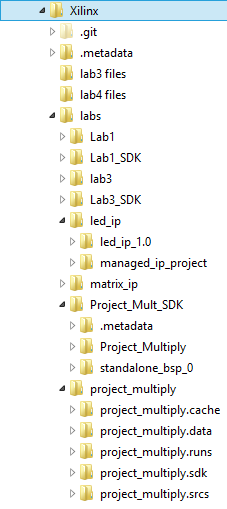
\includegraphics[width=.3\textwidth]{Figures/DirectoryStructure.png}	
\caption{Directory structure}
\label{fig:DirStruct}
\end{center}

\end{figure}


\chapter{Installation}
I am running Windows 8, 64 bit, and using Xilinx software version 2013.4, which is the newest at the moment.\\
The following experiments are defined in: Setting Up a Development Platform for Zynq 2013\_3\_02.pdf

\section{Experiment 1}
\begin{itemize}
	\item Install 7-zip - No comments.
\end{itemize}

\section{Experiment 2}
\begin{itemize}
	\item Register account on Xilinx.com
	\item Download Vivado design suite - appr. 7 Gb
	\item Check it with FastSum, to make sure the MD5 checksum is correct.
	\item Insall Vivado system edition + sdk. Note, the license installion fails, because Windows 8 is not supported. This does not matter.
\end{itemize}

\section{Experiment 3}
\subsection{Install license}
Xilinx license manager does not work in 64 bit mode. Use 32 bit instead!

It is located C:/Xilinx/Vivado/2013.4/ids\_lite/ISE/bin/nt/xlcm.exe

\subsection{Running the Vivado suite}
Vivado GUI is not supported in windows 8! Instead, run the Vivado in Windows 7 compatible mode:

\begin{itemize}
	\item Open C:/Xilinx/Vivado/2013.4/bin/vivado.bat and insert: 
	\item set \_\_COMPAT\_LAYER=WIN7RTM, so the last 3 lines are:
\begin{lstlisting}
	set RDI_PATASK=yes
	set __COMPAT_LAYER=WIN7RTM
	call "%RDI_BINROOT%/loader.bat" -exec %RDI_PROG% %* 
\end{lstlisting}
\end{itemize}

Aparrently, this is not enough. Java throws an exception.

Instead create a new shortcut to the 32 bit program:

\begin{itemize}
	\item Open the folder: 

	C:/Xilinx/Vivado/2013.4/bin/unwrapped/win32.o
	\item Create a shortcut for vivado.exe.
	\item Open the properties for the shortcut.

	\item Change the following:

	\textbf{Target:} = "C:/Xilinx/Vivado/2013.4/bin/unwrapped/win32.o/vvgl.exe C:/Xilinx/Vivado/2013.4/./bin/vivado.bat"

	\textbf{Start in:} = "\%APPDATA\%/Xilinx/Vivado"
\end{itemize}

\section{Experiment 4}
Install USB-UART serial driver

\section{Experiment 5}
Install Tera Term

\section{Experiment 7}
Configure Tera Term
- Note, the virtual com port lost connection: solution = restart PC.

\section{Experiment 8}
Windows firewall

\section{Summary}
Full installation took a couple of hours!\\
This would not be the case on a windows 7 machine.




\chapter{Vivado }
The following steps are defined in: lab1(2)\_EmbeddedSystem.

\section{Hardware Generation}
Step 2-6-4:\\
The GPIO\_0 has disappered. - run step 2-2 and 2-3 again.\\
If it complains about wrong license, with no bitstream generation, just add the right license, WITH bitstream generation.
\newline
\\
Step 3-1-1:\\
lab1.xdc, added in step 2.8 does not work correctly. \\
It seems it is case-sensitive. Correct the lines to:
\begin{lstlisting}
	set_property PACKAGE_PIN R18 [get_ports btnr_tri_io]
	set_property IOSTANDARD LVCMOS25 [get_ports btnr_tri_io]
\end{lstlisting}
\chapter{Xilinx SDK}


\section{Software Platform}
Step 5.1:\\
Building the software platform throws an include error.
\\
Reason: 
\begin{itemize}
	\item There must be NO parentheses or spaces in project path.
	\item The PATH environment variable should be set up properly, by running setting32. This did not work. Instead write the following in the top of the makefile (in one line):
	\\
	PATH=C:/Xilinx/SDK/2013.4/bin/nt;\\
	C:/Xilinx/SDK/2013.4/bin; \\
	C:/Xilinx/SDK/2013.4/gnu/microblaze/nt/bin; \\
	C:/Xilinx/SDK/2013.4/gnu/powerpc-eabi/nt/bin; \\
	C:/Xilinx/SDK/2013.4/gnuwin/bin; \\
	C:/Xilinx/SDK/2013.4/gnu/arm/nt/bin; \\
	C:/Xilinx/SDK/2013.4/gnu/microblaze/linux\_toolchain/nt\_be/bin; \\
	C:/Xilinx/SDK/2013.4/gnu/microblaze/linux\_toolchain/nt\_le/bin;\%PATH\% \\
\end{itemize}

\section{C application}
Step 5.2:\\
Building the C application: \\
Building error: \\
"make: Interrupt/Exception caught (code = 0xc00000fd, addr = 0x4227d3)"\\

This error is caused because of my PATH environment settings. 
It turns out that the ARM gcc compiler uses a file called sh.exe, which is also used/part of the program Github. 
A possible solution is to remove Github from your PATH environment. Or renaming the sh.exe file in github (Then Github might not work!!): C:/Program Files (x86)/Git/bin/sh.exe 	

You might need to restart your PC after changing your PATH variable.

\chapter{Configure Peripherals}
The following exercises and steps are defined in: lab3\_ZynqHW.pdf.
\section{Clocks}
Experiment 2, Step 8: Do not turn of FCLK\_CLK0! It is already in use by the ZYng processor!

\chapter{Create Custom IP}
The following steps are defined in: lab3\_EmbeddedSystem.pdf.
\section{Block design}
Step 4-1-7:\\
Note, the diagrams are not alike, since I did not make Lab2, which is used in the toturial.
There is no BTNR and no leds\_8bits, instead there is btns\_5bits in lab3.
In my design, there is both leds\_8bits and LED[7:0]!\\
The leds\_8bits and BTNR should be removed, and the btns\_5bits should be added!! Otherwise the following lab exercises cannot be completed!\\
This is done by:
\begin{itemize}
	\item Double clicking leds\_8bits and change the board interface to btns\_5bits. Additional the block and external connection should be renamed.
	\item Open the ZYNQ, under MIO Configurations, remove EMIO GPIO.
	\item Delete the BTNR connection from the block design.
	\item Remove the lab1 constraint (and the System\_wrapper constraint), since we deleted BTNR.
\end{itemize}


\chapter{Writing basic software application}
The following steps are defined in: lab4\_EmbeddedSystem.pdf.\\
Note I did not rename my Vivado project, since there is no need to do that!
\newline
\\
Step 2-2: The hw\_platform and bsp will not rebuild automaticly, since the Vivado project has been renamed to lab3, instead of lab1.
Therefore the new hw\_platform must be imported, and the bsp created.
\newline
\\
Step 2-2-15: Note that the LEDs will not light up yet!
\newline
\\
Step 2-4-5: In my case, the correct name is:
\begin{lstlisting}
LED_IP_mWriteReg(XPAR_LED_IP_S_AXI_BASEADDR, 0, dip_check);
\end{lstlisting}
\newline
\\
Step 4-2-2: I do not get any error, because the text area already is in the DDR, and not the BRAM.

\chapter{Console application}
The following steps are defined in: TIHSC1\_Exercise1\_Xilinx.pdf part 3.\\
In the source code given, the defined value for one second should be changed to:
\begin{lstlisting}
#define ONE_SECOND 1333000
\end{lstlisting}

\chapter{Hardware IP Acceleration}
\section{Creating matrix\_ip}
Step 1-2-27 in lab3\_EmbeddedSystem: There is no guide help, thus no "Merge changes....." - I try without...
\newline
\\
Note, that the drivers for matrix\_ip will be located in labs/matrix\_ip/matrix\_ip\_1.0/drivers/matrix\_ip\_v1\_00\_a/src}. For some reason it is not part of the exported hardware platform.


\end{document}